\documentclass{article}
\usepackage[a3paper,landscape,margin=0cm,headheight=0pt,headsep=0pt,footskip=0pt]{geometry}
\usepackage{tikz}
\usetikzlibrary{shapes.multipart,arrows.meta}
\usepackage{graphicx}
\pagestyle{empty}
\setlength{\parindent}{0pt}
\newlength{\diagheight}
\setlength{\diagheight}{0.92\textheight}
\begin{document}
\hbox to \textwidth{%
  \vbox to \textheight{%
    \vfill
    \hbox to 2.5cm{%
      \hfill
      \rotatebox{90}{\large\textbf{Figure 15: DocTIP System Class Diagram}}%
      \hfill
    }%
    \vfill
  }%
  \hfill
  \vbox to \textheight{%
    \vspace*{0.02\textheight}
    \resizebox{!}{\diagheight}{\scalebox{0.8}{
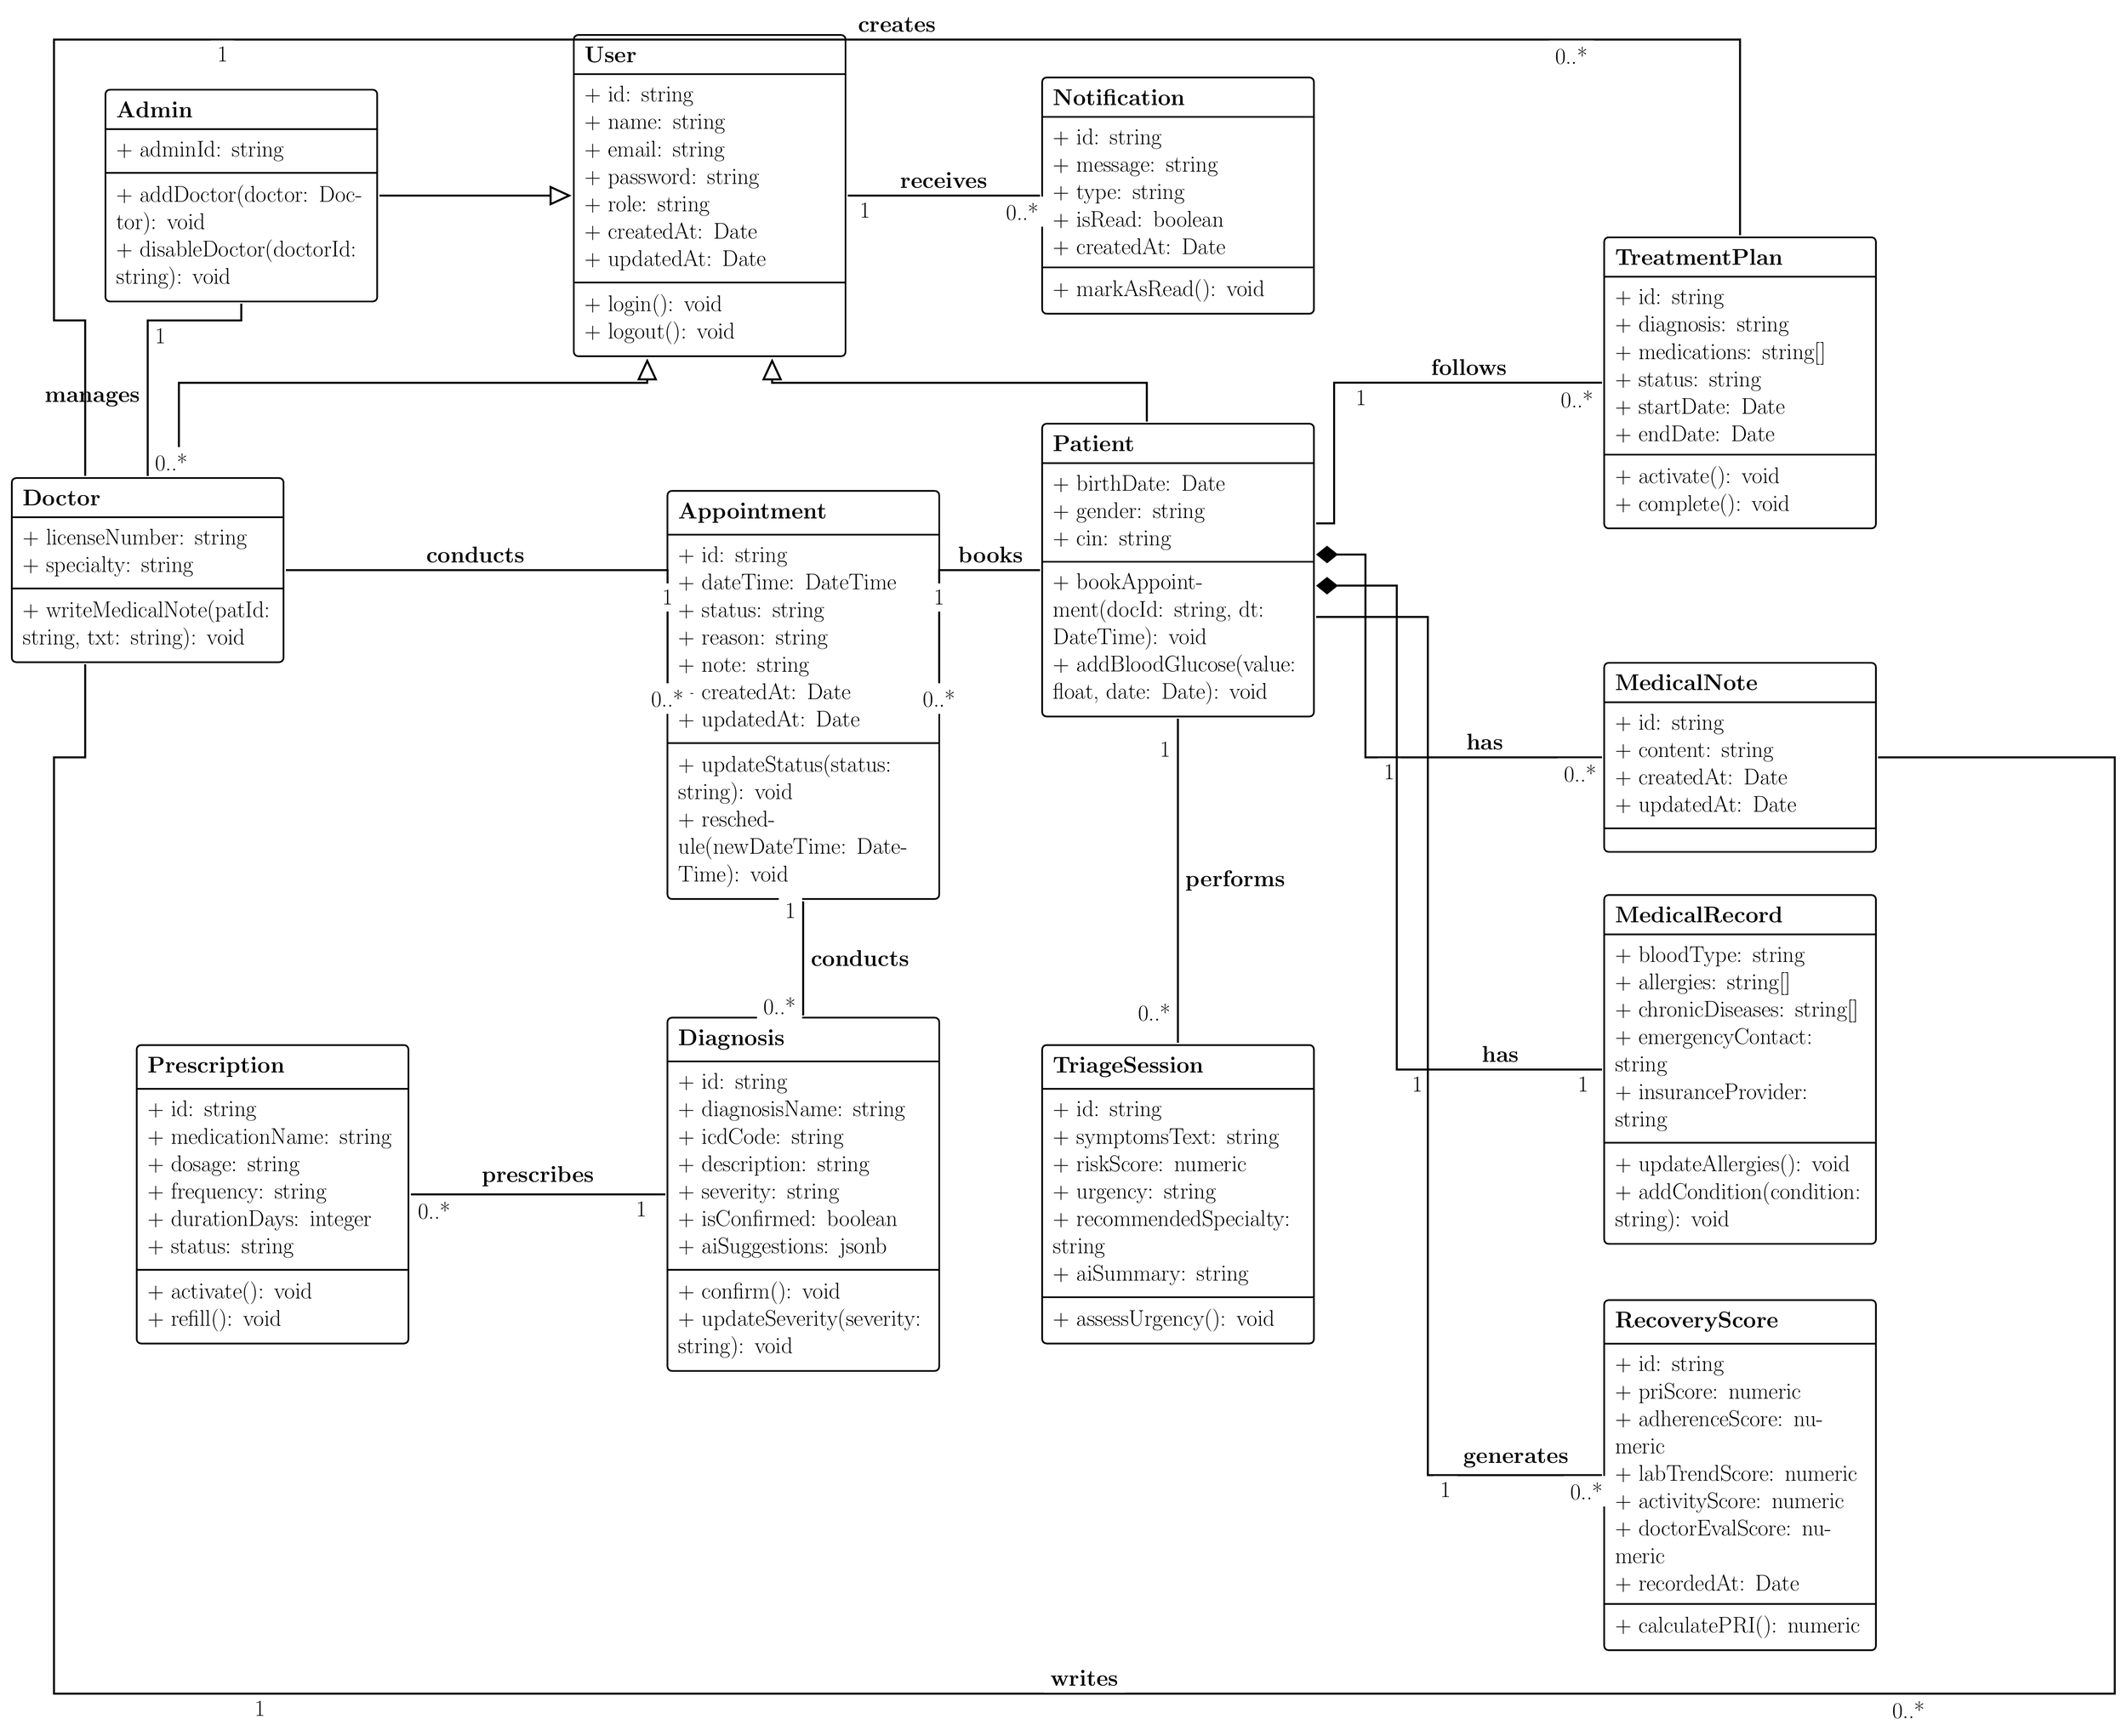
\begin{tikzpicture}[x=1.0cm,y=1.0cm]

  \tikzset{
    class/.style={
      rectangle split,
      rectangle split parts=3,
      rectangle split horizontal=false,
      rectangle split part align={center,left,left},
      draw=black,
      fill=white,
      font=\huge,
      text width=8cm,
      rounded corners=4pt,
      inner sep=10pt,
      outer sep=0pt,
      line width=1.5pt
    },
    inherit/.style={black, line width=1.8pt, shorten >=2pt, shorten <=2pt, -{Triangle[open,fill=white,length=20pt,width=18pt]}},
    assoc/.style={black, line width=1.8pt, shorten >=2pt, shorten <=2pt},
    comp/.style={black, line width=1.8pt, shorten >=2pt, shorten <=2pt, {Diamond[fill=black,length=20pt,width=16pt]}-},
    labeltxt/.style={font=\huge\bfseries, fill=white, inner sep=6pt},
    mult/.style={font=\huge, fill=white, inner sep=6pt}
  }

  \node[class] (admin) at (0, 0) {
    \textbf{Admin}
    \nodepart{second}
    + adminId: string
    \nodepart{third}
    + addDoctor(doctor: Doctor): void\\
    + disableDoctor(doctorId: string): void
  };

  \node[class] (doctor) at (-3, -12) {
    \textbf{Doctor}
    \nodepart{second}
    + licenseNumber: string\\
    + specialty: string
    \nodepart{third}
    + writeMedicalNote(patId: string, txt: string): void
  };

  \node[class] (user) at (15, 0) {
    \textbf{User}
    \nodepart{second}
    + id: string\\
    + name: string\\
    + email: string\\
    + password: string\\
    + role: string\\
    + createdAt: Date\\
    + updatedAt: Date
    \nodepart{third}
    + login(): void\\
    + logout(): void
  };

  \node[class] (appointment) at (18, -16) {
    \textbf{Appointment}
    \nodepart{second}
    + id: string\\
    + dateTime: DateTime\\
    + status: string\\
    + reason: string\\
    + note: string\\
    + createdAt: Date\\
    + updatedAt: Date
    \nodepart{third}
    + updateStatus(status: string): void\\
    + reschedule(newDateTime: DateTime): void
  };

  \node[class] (diagnosis) at (18, -32) {
    \textbf{Diagnosis}
    \nodepart{second}
    + id: string\\
    + diagnosisName: string\\
    + icdCode: string\\
    + description: string\\
    + severity: string\\
    + isConfirmed: boolean\\
    + aiSuggestions: jsonb
    \nodepart{third}
    + confirm(): void\\
    + updateSeverity(severity: string): void
  };

  \node[class] (prescription) at (1, -32) {
    \textbf{Prescription}
    \nodepart{second}
    + id: string\\
    + medicationName: string\\
    + dosage: string\\
    + frequency: string\\
    + durationDays: integer\\
    + status: string
    \nodepart{third}
    + activate(): void\\
    + refill(): void
  };

  \node[class] (notification) at (30, 0) {
    \textbf{Notification}
    \nodepart{second}
    + id: string\\
    + message: string\\
    + type: string\\
    + isRead: boolean\\
    + createdAt: Date
    \nodepart{third}
    + markAsRead(): void
  };

  \node[class] (patient) at (30, -12) {
    \textbf{Patient}
    \nodepart{second}
    + birthDate: Date\\
    + gender: string\\
    + cin: string
    \nodepart{third}
    + bookAppointment(docId: string, dt: DateTime): void\\
    + addBloodGlucose(value: float, date: Date): void
  };

  \node[class] (triageSession) at (30, -32) {
    \textbf{TriageSession}
    \nodepart{second}
    + id: string\\
    + symptomsText: string\\
    + riskScore: numeric\\
    + urgency: string\\
    + recommendedSpecialty: string\\
    + aiSummary: string
    \nodepart{third}
    + assessUrgency(): void
  };

  \node[class] (treatmentPlan) at (48, -6) {
    \textbf{TreatmentPlan}
    \nodepart{second}
    + id: string\\
    + diagnosis: string\\
    + medications: string[]\\
    + status: string\\
    + startDate: Date\\
    + endDate: Date
    \nodepart{third}
    + activate(): void\\
    + complete(): void
  };

  \node[class] (medicalNote) at (48, -18) {
    \textbf{MedicalNote}
    \nodepart{second}
    + id: string\\
    + content: string\\
    + createdAt: Date\\
    + updatedAt: Date
    \nodepart{third}
  };

  \node[class] (medicalRecord) at (48, -28) {
    \textbf{MedicalRecord}
    \nodepart{second}
    + bloodType: string\\
    + allergies: string[]\\
    + chronicDiseases: string[]\\
    + emergencyContact: string\\
    + insuranceProvider: string
    \nodepart{third}
    + updateAllergies(): void\\
    + addCondition(condition: string): void
  };

  \node[class] (recoveryScore) at (48, -41) {
    \textbf{RecoveryScore}
    \nodepart{second}
    + id: string\\
    + priScore: numeric\\
    + adherenceScore: numeric\\
    + labTrendScore: numeric\\
    + activityScore: numeric\\
    + doctorEvalScore: numeric\\
    + recordedAt: Date
    \nodepart{third}
    + calculatePRI(): numeric
  };

  % ===================================
  % INHERITANCE LINES
  % ===================================
  \draw[inherit] (admin.east) -- (user.west);
  \draw[inherit] ([xshift=1cm]doctor.north) -- (-2, -6) -- (13, -6) -- ([xshift=-2cm]user.south);
  \draw[inherit] ([xshift=-1cm]patient.north) -- (29, -6) -- (17, -6) -- ([xshift=2cm]user.south);

  % ===================================
  % ASSOCIATION LINES (all orthogonal)
  % ===================================
  % admin manages doctor
  \draw[assoc] (admin.south) -- (0, -4) -- (-3, -4) -- node[labeltxt, left] {manages} node[mult, right, pos=0.1] {1} node[mult, right, pos=0.9] {0..*} (doctor.north);

  % user receives notification
  \draw[assoc] (user.east) -- node[labeltxt, above] {receives} node[mult, below, pos=0.1] {1} node[mult, below, pos=0.9] {0..*} (notification.west);

  % patient books appointment (orthogonal)
  \draw[assoc] (patient.west) -- node[labeltxt, above] {books} (patient.west -| appointment.east) -- node[mult, below, pos=0.1] {1} node[mult, below, pos=0.9] {0..*} (appointment.east);

  % doctor conducts appointment (orthogonal)
  \draw[assoc] (doctor.east) -- node[labeltxt, above] {conducts} (doctor.east -| appointment.west) -- node[mult, below, pos=0.1] {1} node[mult, below, pos=0.9] {0..*} (appointment.west);

  % appointment conducts diagnosis (vertical)
  \draw[assoc] (appointment.south) -- node[labeltxt, right] {conducts} node[mult, left, pos=0.1] {1} node[mult, left, pos=0.9] {0..*} (diagnosis.north);

  % diagnosis prescribes prescription (horizontal)
  \draw[assoc] (diagnosis.west) -- node[labeltxt, above] {prescribes} node[mult, below, pos=0.1] {1} node[mult, below, pos=0.9] {0..*} (prescription.east);

  % patient performs triageSession (vertical)
  \draw[assoc] (patient.south) -- node[labeltxt, right] {performs} node[mult, left, pos=0.1] {1} node[mult, left, pos=0.9] {0..*} (triageSession.north);

  % ===================================
  % RIGHT-SIDE LINES FROM PATIENT
  % ===================================
  \draw[assoc] ([yshift=1.5cm]patient.east) -- (35, -10.5) -- (35, -6) -- node[labeltxt, above] {follows} node[mult, below, pos=0.1] {1} node[mult, below, pos=0.9] {0..*} (treatmentPlan.west);
  \draw[comp] ([yshift=0.5cm]patient.east) -- (36, -11.5) -- (36, -18) -- node[labeltxt, above] {has} node[mult, below, pos=0.1] {1} node[mult, below, pos=0.9] {0..*} (medicalNote.west);
  \draw[comp] ([yshift=-0.5cm]patient.east) -- (37, -12.5) -- (37, -28) -- node[labeltxt, above] {has} node[mult, below, pos=0.1] {1} node[mult, below, pos=0.9] {1} (medicalRecord.west);
  \draw[assoc] ([yshift=-1.5cm]patient.east) -- (38, -13.5) -- (38, -41) -- node[labeltxt, above] {generates} node[mult, below, pos=0.1] {1} node[mult, below, pos=0.9] {0..*} (recoveryScore.west);

  % ===================================
  % DOCTOR TO RIGHT-SIDE LINES (orthogonal, below all boxes)
  % ===================================
  % doctor creates treatmentPlan
  \draw[assoc] ([xshift=-2cm]doctor.north) -- (-5, -4) -- (-6, -4) -- (-6, 5) -- node[labeltxt, above] {creates} node[mult, below, pos=0.1] {1} node[mult, below, pos=0.9] {0..*} (48, 5) -- (treatmentPlan.north);

  % doctor writes medicalNote
  \draw[assoc] ([xshift=-2cm]doctor.south) -- (-5, -18) -- (-6, -18) -- (-6, -48) -- node[labeltxt, above, pos=0.5] {writes} node[mult, below, pos=0.1] {1} node[mult, below, pos=0.9] {0..*} (60, -48) -- (60, -18) -- (medicalNote.east);

\end{tikzpicture}
}
}%
    \vfill
  }%
}
\end{document}
